% ============================================================
% Final Project Presentation
% Project 17: Multimodal Question Answering (VQA)
% Course: CSC15012 - Applications of NLP in Industry
% Student: Le Dinh Minh Quan - 23127460 - 23CNTThuc
% Template: Beamer (Madrid + seahorse, aspectratio=169)
% ============================================================

\documentclass[10pt,aspectratio=169]{beamer}

\mode<presentation>
{
  \usetheme{Madrid}
  \usecolortheme{seahorse}
  \usefonttheme{default}
  \setbeamertemplate{navigation symbols}{}
  \setbeamertemplate{caption}[numbered]
  \setbeamertemplate{footline}[frame number]
}

% ---- Packages ----
\usepackage[english]{babel}
\usepackage[utf8]{inputenc}
\usepackage{amsmath}
\usepackage{amssymb}
\usepackage{graphicx}
\usepackage{booktabs}
\usepackage{xcolor}
\usepackage{hyperref}
\usepackage{xurl}
\usepackage{tikz}
\usepackage{pgfplots}
\pgfplotsset{compat=1.18}
\usetikzlibrary{shapes.geometric, arrows.meta, positioning, fit, backgrounds, shadows}
\usepackage{listings}
\lstset{
  basicstyle=\ttfamily\scriptsize,
  breaklines=true,
  frame=single,
  backgroundcolor=\color{gray!10},
  keywordstyle=\color{blue},
  commentstyle=\color{green!60!black},
  stringstyle=\color{red!70!black},
  showstringspaces=false,
  tabsize=2
}

% ---- HCMUS LOGO ----
% Upload logo_hcmus.png to Overleaf to display the logo (top-right of every slide).
% If the file is missing, no logo is shown (no error).
\IfFileExists{logo_hcmus.png}{\logo{\includegraphics[height=0.7cm]{logo_hcmus.png}}}{}

% ---- TITLE METADATA ----
\title[Project 17: Multimodal QA (VQA)]{Project 17: Multimodal Question Answering (VQA)}
\subtitle{A Trainable ViLT Core behind a Type-Aware, Abstaining Agent}
\author[Le Dinh Minh Quan]{Le Dinh Minh Quan \\ \small ID: 23127460 -- Class: 23CNTThuc}
\institute[HCMUS]{Vietnam National University Ho Chi Minh City \\ University of Science -- Faculty of Information Technology \\ \small Course: CSC15012 -- Applications of NLP in Industry}
\date{2026}

\begin{document}

% ============================================================
% SLIDE 1: TITLE
% ============================================================
\begin{frame}
  \titlepage
\end{frame}

% ============================================================
% SLIDE 2: OUTLINE
% ============================================================
\begin{frame}{Outline}
\begin{columns}[T]
\begin{column}{0.5\textwidth}
\begin{enumerate}
  \item Business Problem \& Motivation
  \item Proposed NLP Solution \& Success Metrics
  \item System Architecture (Serving)
  \item Repository \& Tech Stack
  \item Data Overview
  \item Training \& Autopilot Workflow
  \item Model Selection \& VQA Metric
  \item Evaluation Results \& Baselines
\end{enumerate}
\end{column}
\begin{column}{0.5\textwidth}
\begin{enumerate}
  \setcounter{enumi}{8}
  \item Agentic AI Component (D1--D5)
  \item Example Interactions
  \item Deployment
  \item Ethics, Privacy \& Fairness
  \item Monitoring \& Continual Learning
  \item Key Takeaways \& Future Work
  \item Resources \& Thank You
\end{enumerate}
\end{column}
\end{columns}
\end{frame}

% ============================================================
% SLIDE 3: BUSINESS PROBLEM & MOTIVATION
% ============================================================
\begin{frame}{1. Business Problem \& Motivation}
\begin{block}{Context}
Visual Question Answering: given an \texttt{(image, question)} pair, return a short answer (``how many chairs?'' $\rightarrow$ ``2''). The answer must be \textbf{grounded in the image} -- answering ``yellow'' to ``what color is the banana?'' \emph{without looking} is just a language prior.
\end{block}

\begin{columns}[T]
\begin{column}{0.5\textwidth}
\textbf{Why it is hard}
\begin{itemize}\small
  \item Two modalities, one answer (fuse pixels + tokens)
  \item Open-ended questions $\rightarrow$ different answer kinds
  \item Models are \textbf{overconfident} and prior-driven
  \item A bare model cannot say ``I don't know''
\end{itemize}
\end{column}
\begin{column}{0.5\textwidth}
\textbf{Stakeholders}
\begin{itemize}\small
  \item Blind / low-vision users (VizWiz, high stakes)
  \item E-commerce product Q\&A
  \item Image search \& retrieval
  \item Content-moderation triage
  \item Developers (REST API)
\end{itemize}
\end{column}
\end{columns}
\end{frame}

% ============================================================
% SLIDE 4: PROPOSED NLP SOLUTION + SUCCESS METRICS
% ============================================================
\begin{frame}{2. Proposed NLP Solution \& Success Metrics}
\begin{block}{Solution (\texttt{mmqa})}
A \textbf{trainable ViLT VQA core} (\texttt{dandelin/vilt-b32-finetuned-vqa}, Apache-2.0) behind a deterministic \textbf{agent (D1--D5)} that classifies the question type, runs the model, \textbf{abstains when uncertain}, and \textbf{constrains} the answer to the type. Only the VQA model is trained.
\end{block}

\begin{table}[h]
\centering\small
\begin{tabular}{lll}
\toprule
\textbf{Type} & \textbf{Metric} & \textbf{Reads as} \\
\midrule
Technical & Official VQA soft accuracy (per type) & Beat 4 bias baselines \\
Technical & Image-contribution gap (full $-$ blind) & Large gap $=$ image is used \\
Technical & Answer-when-confident acc vs raw argmax & Higher precision, coverage $<$1 \\
Technical & Re-rank rate (D5 activity) & Fixes type-wrong argmax \\
Safety & ``Unsure'' instead of wrong answer & Abstain when uncertain \\
\bottomrule
\end{tabular}
\end{table}

\textbf{Verified offline (synthetic spine):} model accuracy \textbf{1.0} vs blind prior \textbf{0.26}, per-type all 1.0, coverage 1.0, all 5 decisions fire, \textbf{grade 1.0}, 27 tests pass -- a code-path guarantee; honest numbers come from the real ViLT on \texttt{lmms-lab/VQAv2} via Colab H100.
\end{frame}

% ============================================================
% SLIDE 5: SYSTEM ARCHITECTURE (Serving, TikZ)
% ============================================================
\begin{frame}{3. System Architecture (Serving Topology)}
\centering
\resizebox{0.98\linewidth}{!}{%
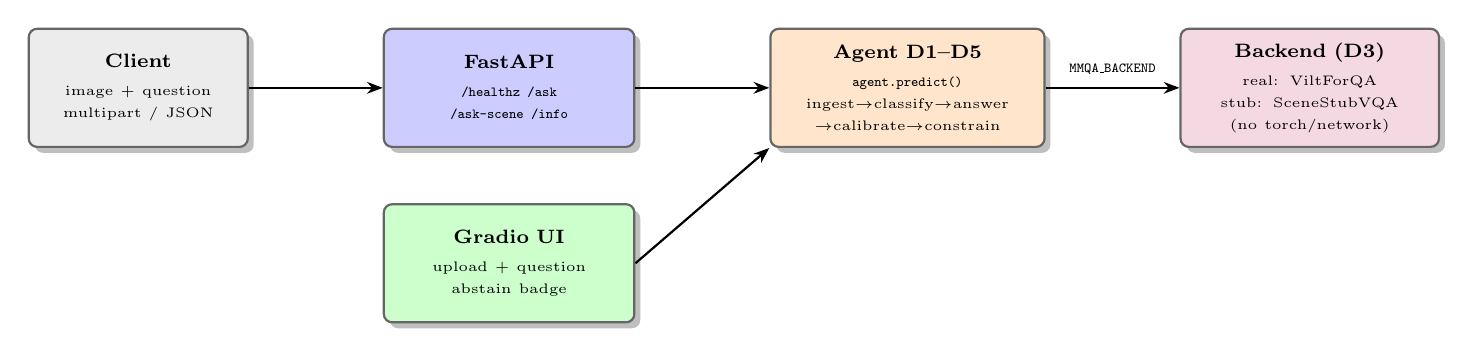
\begin{tikzpicture}[
  node distance=0.7cm and 1.7cm,
  box/.style={rectangle, draw=black!60, rounded corners=3pt, thick,
              text width=2.9cm, minimum height=1.5cm, align=center,
              inner sep=4pt, font=\scriptsize, drop shadow},
  inbox/.style={box, fill=gray!15, text width=2.5cm},
  apibox/.style={box, fill=blue!20},
  uibox/.style={box, fill=green!20},
  agentbox/.style={box, fill=orange!20, text width=3.2cm},
  modelbox/.style={box, fill=purple!15, text width=3.0cm},
  arrow/.style={-{Stealth[length=2mm]}, thick}
]
\node[inbox] (user) {\textbf{Client}\\[2pt]{\tiny image + question}\\{\tiny multipart / JSON}};
\node[apibox, right=of user] (api) {\textbf{FastAPI}\\[2pt]{\tiny \texttt{/healthz} \texttt{/ask}}\\{\tiny \texttt{/ask-scene} \texttt{/info}}};
\node[uibox, below=of api] (ui) {\textbf{Gradio UI}\\[2pt]{\tiny upload + question}\\{\tiny abstain badge}};
\node[agentbox, right=of api] (agent) {\textbf{Agent D1--D5}\\[2pt]{\tiny \texttt{agent.predict()}}\\{\tiny ingest$\to$classify$\to$answer}\\{\tiny $\to$calibrate$\to$constrain}};
\node[modelbox, right=of agent] (model) {\textbf{Backend (D3)}\\[2pt]{\tiny real: ViltForQA}\\{\tiny stub: SceneStubVQA}\\{\tiny (no torch/network)}};
\draw[arrow] (user) -- (api);
\draw[arrow] (ui.east) -- (agent.south west);
\draw[arrow] (api) -- (agent);
\draw[arrow] (agent) -- node[above=1pt,font=\tiny]{\texttt{MMQA\_BACKEND}} (model);
\end{tikzpicture}%
}

\vspace{0.2cm}
\scriptsize \textbf{One inference path}: API and UI are thin adapters over the same \texttt{agent.predict()}. A single env var selects the real ViLT or the torch-free \texttt{SceneStubVQA} -- swapping the stub for the real wrapper flips to production with \textbf{no agent changes}. The served default is the clean Apache-2.0 ViLT.
\end{frame}

% ============================================================
% SLIDE 6: REPOSITORY & TECH STACK
% ============================================================
\begin{frame}[fragile]{4. Repository Structure \& Tech Stack}
\begin{columns}[T]
\begin{column}{0.56\textwidth}
\textbf{GitHub repo} (public, MIT) \\
\scriptsize \url{https://github.com/ledinhminhquan/17_Multimodal_QA}

\vspace{0.15cm}
\begin{lstlisting}[basicstyle=\ttfamily\tiny]
17_Multimodal_QA/
|-- src/mmqa/
|   |-- config cli logging_utils
|   |-- data/      # synth_scene generator + answerer
|   |-- models/    # vqa_model (ViLT/BLIP/SceneStub),
|   |              #   question_type, baseline, registry
|   |-- vision/    # image_utils + SceneImage carrier
|   |-- training/  # train_vqa, evaluate, tune, metrics
|   |-- agent/     # state, policy (D1-D5), tools, brain
|   |-- api/       # FastAPI main, ui (Gradio)
|   |-- analysis/ autoreport/ monitoring/
|   |-- automation/ (autopilot)  grading/ (checklist)
|-- configs/  docs/ (14 + DESIGN_BRIEF)  notebooks/
|-- app/ deploy/ sample_data/ scripts/ tests/
|-- Dockerfile  docker-compose.yml  Makefile
+-- LICENSE (MIT)  README.md  ci.yml
\end{lstlisting}
\end{column}
\begin{column}{0.44\textwidth}
\textbf{Tech stack}
\begin{itemize}\small
  \item Python 3.11/3.12, Git + GitHub
  \item PyTorch + HF Transformers
  \item \textbf{ViLT} \texttt{vilt-b32-finetuned-vqa} (113M, Apache)
  \item Vocab: ViLT \texttt{id2label} (3129)
  \item \texttt{ViltProcessor} (384px + WordPiece)
  \item BLIP / GIT (generative alt.)
  \item FastAPI + Uvicorn, Gradio
  \item Docker + compose (libGL)
  \item Synthetic scenes + \texttt{SceneStubVQA}
  \item Colab T4 $\rightarrow$ A100/L4 $\rightarrow$ H100
\end{itemize}
\end{column}
\end{columns}
\end{frame}

% ============================================================
% SLIDE 7: DATA OVERVIEW
% ============================================================
\begin{frame}{5. Data Overview}
\begin{columns}[T]
\begin{column}{0.52\textwidth}
\textbf{Sources (verified on HF Hub)}
\begin{itemize}\scriptsize
  \item \textbf{EVAL}: \texttt{lmms-lab/VQAv2} val (214.4K), \textbf{cc-by-4.0}, 8 cols, 10 annotators
  \item \textbf{TRAIN}: \texttt{HuggingFaceM4/VQAv2} ($\sim$443K) -- \textbf{FLAG}, \texttt{trust\_remote\_code}, fragile
  \item \textbf{TINY/offline}: \texttt{Multimodal-Fatima/} \texttt{VQAv2\_sample\_train} (1K, full schema, FLAG)
  \item \textbf{DEMO}: \texttt{merve/vqav2-small} (3 cols, FLAG -- not valid for scoring)
  \item \textbf{VOCAB}: ViLT config (3129, Apache)
\end{itemize}
\textbf{License hygiene}: prefer declared-clean (VQAv2 cc-by-4.0, GQA mit, ViLT apache); FLAG undeclared mirrors; \textbf{avoid} \texttt{daquar\_vqa} (cc-by-nc-sa).
\end{column}
\begin{column}{0.48\textwidth}
\textbf{Synthetic scene generator (offline spine)}
\begin{itemize}\scriptsize
  \item \texttt{make\_scene(seed)}: shapes $\times$ 6 colors on PIL canvas
  \item Embeds \texttt{scene\_spec} in PNG metadata $\rightarrow$ self-describing, deterministic
  \item Templates yes\_no / count / color / object + a 10-answer list
  \item \texttt{SceneStubVQA} returns a \textbf{realistic} top-$k$ ($\sim$0.7--0.9 on truth) + difficulty knob
\end{itemize}
\textbf{The 10-annotator structure} drives the official soft accuracy
\[
\mathrm{acc}(a)=\min\!\Big(1,\tfrac{\#\text{matches}}{3}\Big)
\]
A dataset without 10 annotators cannot produce this score (why \texttt{merve} is demo-only).
\end{column}
\end{columns}
\end{frame}

% ============================================================
% SLIDE 8: TRAINING & AUTOPILOT WORKFLOW (TikZ)
% ============================================================
\begin{frame}{6. Training \& Autopilot Workflow (Colab H100)}
\centering
\begin{tikzpicture}[
  node distance=0.16cm,
  step/.style={rectangle, draw=black!60, rounded corners=2pt, thick,
              minimum width=11.6cm, minimum height=0.5cm, align=center, font=\scriptsize},
  setup/.style={step, fill=gray!15},
  train/.style={step, fill=orange!15},
  eval/.style={step, fill=blue!15},
  deploy/.style={step, fill=green!15},
  arrow/.style={-{Stealth[length=1.6mm]}, thick}
]
\node[setup] (s1) {\textbf{1. Setup}: re-verify HF ids+licenses, pull 3129 vocab (\texttt{len==3129})};
\node[setup, below=of s1] (s2) {\textbf{2. Synthetic scenes + stub}: self-describing PNGs; assert all 5 decisions fire};
\node[train, below=of s2] (s3) {\textbf{3. Fine-tune ViLT} on VQAv2 train (resume-safe, T4/A100/H100-adaptive)};
\node[eval, below=of s3] (s4) {\textbf{4. Evaluation}: soft VQA acc on \texttt{lmms-lab/VQAv2} val (overall + per-type)};
\node[eval, below=of s4] (s5) {\textbf{5. Baselines}: prior-yes, per-type prior, \textbf{blind question-only}, zero-shot ViLT};
\node[eval, below=of s5] (s6) {\textbf{6. Calibrate D4} (temperature scaling) + abstention/coverage + re-rank + risk--coverage};
\node[deploy, below=of s6] (s7) {\textbf{7. Auto-gen} report PDF + slides PPTX};
\node[deploy, below=of s7] (s8) {\textbf{8. Grade + bundle} (\texttt{grading/checklist.py}: verified \textbf{grade 1.0})};
\foreach \a/\b in {s1/s2,s2/s3,s3/s4,s4/s5,s5/s6,s6/s7,s7/s8}
  \draw[arrow] (\a) -- (\b);
\end{tikzpicture}

\vspace{0.12cm}
\scriptsize \textbf{One-button Run-All}. Auto-resume on disconnect. Hardware-adaptive (ViLT 113M fine-tunes even on free T4 @384px; H100 unlocks BLIP-2/Qwen via bf16+LoRA). Offline-first: the synthetic path runs the whole pipeline torch-free in CI.
\end{frame}

% ============================================================
% SLIDE 9: MODEL SELECTION & VQA METRIC
% ============================================================
\begin{frame}{7. Model Selection \& the VQA Metric}
\begin{columns}[T]
\begin{column}{0.52\textwidth}
\textbf{Classification (DEFAULT) vs generative}
\begin{table}[h]
\centering\scriptsize
\begin{tabular}{lcc}
\toprule
 & \textbf{Class. (ViLT)} & \textbf{Gen. (BLIP)} \\
\midrule
Vocab & fixed 3129 & open \\
Confidence & clean softmax & logprob proxy \\
Params & $\sim$113M & $\sim$385M \\
Ceiling & OOV unreachable & none \\
\bottomrule
\end{tabular}
\end{table}
\scriptsize \textbf{Why ViLT classification}: cleanest \texttt{p\_max}/margin/entropy for D4; 3129 vocab already holds yes/no, ints, colors (D5 = filtered argmax); Apache-2.0; smallest core that fully fine-tunes on a free T4; already the vocab source.

\vspace{0.1cm}
\scriptsize \textbf{FLAG / avoid}: \texttt{pix2struct-vqav2-base} (404); \texttt{llava-1.5-7b} (llama2 NC); \texttt{Qwen2.5-VL-3B} (Qwen Research NC) -- upper-bound only.
\end{column}
\begin{column}{0.48\textwidth}
\textbf{Official VQA soft accuracy} (no HF metric exists $\rightarrow$ re-implemented \texttt{VQAEval})
\[
\mathrm{acc}(a)=\min\!\Big(1,\tfrac{\#\text{of 10 annot. matching}}{3}\Big)
\]
\begin{itemize}\scriptsize
  \item Full \textbf{10$\times$ leave-one-out} average (not the simplification)
  \item \textbf{One canonical normalizer} for prediction \emph{and} all 10 GT: lowercase; keep \texttt{2.5}; \texttt{100,000}$\to$\texttt{100000}; word$\to$digit; drop \texttt{a/an/the}; $\sim$80 contractions
  \item Report \textbf{per-answer-type} (yes/no, number, other) + per-question-type (65)
  \item Typical ordering: yes/no highest, number lowest
\end{itemize}
\end{column}
\end{columns}
\end{frame}

% ============================================================
% SLIDE 10: EVALUATION RESULTS & BASELINES
% ============================================================
\begin{frame}{8. Evaluation Results \& Baseline Ladder}
\begin{columns}[T]
\begin{column}{0.5\textwidth}
\textbf{Verified offline (SceneStubVQA)} -- a \emph{code-path / plumbing} check, not a model result
\begin{table}[h]
\centering\scriptsize
\begin{tabular}{lc}
\toprule
\textbf{Quantity} & \textbf{Offline} \\
\midrule
Model VQA accuracy & \textbf{1.0} \\
Blind question-only prior & 0.26 \\
Per-type (4 types) & all 1.0 \\
Agent coverage & 1.0 \\
Decisions firing (D1--D5) & all 5 \\
Automated grade & \textbf{1.0} \\
Unit tests passing & 27 \\
\bottomrule
\end{tabular}
\end{table}
\scriptsize Offline 1.0 is the \textbf{perfect-scene-reading upper bound}; honest numbers come from the real ViLT on VQAv2 (Colab H100).
\end{column}
\begin{column}{0.5\textwidth}
\textbf{Image contribution} (full $-$ blind) on the spine
\begin{center}
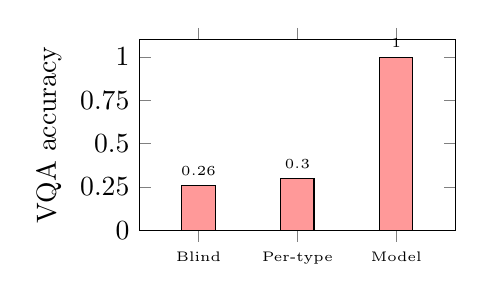
\begin{tikzpicture}
\begin{axis}[
  ybar, width=5.6cm, height=4.0cm,
  ymin=0, ymax=1.1,
  symbolic x coords={Blind, Per-type, Model},
  xtick=data,
  ylabel={VQA accuracy},
  bar width=12pt,
  nodes near coords, nodes near coords style={font=\tiny},
  enlarge x limits=0.3,
  ytick={0,0.25,0.5,0.75,1.0},
  x tick label style={font=\tiny}
]
\addplot[fill=red!40] coordinates {(Blind,0.26) (Per-type,0.30) (Model,1.0)};
\end{axis}
\end{tikzpicture}
\end{center}
\scriptsize The \textbf{model 1.0 vs blind 0.26} gap proves the system uses the \emph{image}, not just language priors -- the load-bearing ``does it look at the picture'' signal.
\end{column}
\end{columns}
\end{frame}

% ============================================================
% SLIDE 11: AGENTIC AI COMPONENT (D1-D5, TikZ)
% ============================================================
\begin{frame}{9. Agentic AI Component -- 5-Decision FSM}
\centering
\begin{tikzpicture}[
  node distance=0.16cm,
  step/.style={rectangle, draw=black!60, rounded corners=2pt, thick,
              text width=11.6cm, minimum height=0.5cm, align=center, font=\scriptsize, inner sep=3pt},
  gate/.style={step, fill=gray!15},
  route/.style={step, fill=blue!12},
  model/.style={step, fill=purple!15},
  decide/.style={step, fill=red!12},
  cons/.style={step, fill=green!15},
  arrow/.style={-{Stealth[length=1.6mm]}, thick}
]
\node[gate] (d1) {\textbf{D1 INGEST} (\textbf{tool}, no torch): valid RGB image (var$>$eps) AND interrogative question $\to$ else HALT \texttt{error:bad\_image/question}};
\node[route, below=of d1] (d2) {\textbf{D2 CLASSIFY} (\textbf{multi-step reasoning}): \texttt{is/are}$\to$yes\_no \;|\; \texttt{how many}$\to$count \;|\; \texttt{what color}$\to$color \;|\; else object/other};
\node[model, below=of d2] (d3) {\textbf{D3 ANSWER} (\textbf{tool}, only model call): ViltForQA logits | SceneStubVQA $\to$ topk, p\_max, margin, entropy (exc.$\to$\texttt{error:model\_failure})};
\node[decide, below=of d3] (d4) {\textbf{D4 CALIBRATE} (\textbf{decision-making}): p\_max$\geq\tau_c$ AND margin$\geq\tau_m$ AND entropy$\leq\tau_e$ (temp-scaled, per-type) $\to$ else \texttt{"unsure"} abstain};
\node[cons, below=of d4] (d5) {\textbf{D5 CONSTRAIN} (\textbf{decision-making}): top-$k$ in allowed type set $\to$ \texttt{ok} | re-rank $\to$ \texttt{ok:reranked} | none $\to$ \texttt{abstained:type\_mismatch}};
\foreach \a/\b in {d1/d2,d2/d3,d3/d4,d4/d5}
  \draw[arrow] (\a) -- (\b);
\end{tikzpicture}

\vspace{0.12cm}
\scriptsize Only \textbf{D3} touches the model; D1/D2/D4/D5 are deterministic logic over the model's own top-$k$. Implements \textbf{multi-step reasoning} (D2,D4,D5), \textbf{tool usage} (D1,D3), \textbf{decision-making on intermediate outputs} (D4,D5). Value-add over raw argmax with \textbf{no extra training}: calibrated abstention + type-aware constraint. Optional LLM brain is advisory-only, OFF by default, \emph{never overrides}.
\end{frame}

% ============================================================
% SLIDE 12: DECISION TABLE + EXAMPLE INTERACTIONS
% ============================================================
\begin{frame}[fragile]{10. Decision Table \& Example Traces}
\begin{table}[h]
\centering\scriptsize
\begin{tabular}{clll}
\toprule
\textbf{D} & \textbf{Stage} & \textbf{Gates on} & \textbf{Branches} \\
\midrule
D1 & Ingest & valid image + interrogative question & ok / \texttt{error:bad\_image|question} \\
D2 & Classify & leading keyword (first-match-wins) & yes\_no / count / color / object \\
D3 & Answer & model $\to$ topk, p\_max, margin, entropy & ok / \texttt{error:model\_failure} \\
D4 & Calibrate & p\_max $\wedge$ margin $\wedge$ entropy & confident / \texttt{abstained:low\_confidence} \\
D5 & Constrain & top-$k$ $\in$ allowed type set & ok / ok:reranked / type\_mismatch \\
\bottomrule
\end{tabular}
\end{table}

\begin{lstlisting}[basicstyle=\ttfamily\tiny]
# A -- clean count, re-ranked to type (3 red squares)
Q: "how many red squares?"
 D2 count ; D3 topk=[("squares",.41),("3",.33),("2",.14),...]
 D4 temp-cal p_max .47>=.45, margin .12>=.10 -> CONFIDENT
 D5 "squares" not a count -> scan -> "3"
 -> answer="3" status=ok:reranked  (raw argmax would score 0)

# B -- low confidence, abstain (ambiguous triangle color)
Q: "what color is the triangle?"
 D3 topk=[("red",.28),("orange",.24),("blue",.20),...] margin .04 entropy 1.59
 D4 fails all three -> answer="unsure" status=abstained:low_confidence needs_review=true
\end{lstlisting}
\end{frame}

% ============================================================
% SLIDE 13: DEPLOYMENT
% ============================================================
\begin{frame}[fragile]{11. Deployment (4 formats over one path)}
\begin{columns}[T]
\begin{column}{0.52\textwidth}
\textbf{Formats}
\begin{itemize}\scriptsize
  \item \textbf{REST API} (FastAPI): \texttt{/healthz} \texttt{/ask} (multipart image+question) \texttt{/ask-scene} (JSON) \texttt{/info}
  \item \textbf{Gradio UI}: upload + question + confidence bar + abstain badge + top-$k$ table
  \item \textbf{Docker}: Dockerfile + compose (\texttt{libGL} for Pillow)
  \item \textbf{Colab H100 autopilot}: one-button fine-tune $\to$ report
\end{itemize}
\scriptsize \textbf{HTTP map}: \texttt{ok}/\texttt{ok:reranked}/both \texttt{abstained:*} $\to$ 200; bad input $\to$ 422; model failure $\to$ 500.

\scriptsize \textbf{Honesty}: deployable, but \emph{not} currently on a public URL.
\end{column}
\begin{column}{0.48\textwidth}
\textbf{Config (env vars)}
\begin{lstlisting}[basicstyle=\ttfamily\tiny]
MMQA_BACKEND=stub|vilt
MMQA_MODEL_ID=dandelin/vilt-b32-finetuned-vqa
MMQA_DEVICE=cpu|cuda   # CPU fallback if no CUDA
MMQA_TOP_K=5
MMQA_TAU_CONF=0.30 TAU_ENT=1.5 TAU_MARGIN=0.10
MMQA_TEMPERATURE=1.0   # tuned on held-out split
MMQA_RETAIN_IMAGES=false   # privacy default
MMQA_ENABLE_LLM=false      # brain OFF
\end{lstlisting}
\scriptsize ViLT is small ($\sim$113M) -- a \textbf{T4 serves it}; no A100/H100 needed to serve. Two Docker flavours: small CPU/stub (Pillow only) and GPU/real ViLT.
\end{column}
\end{columns}
\end{frame}

% ============================================================
% SLIDE 14: ETHICS, PRIVACY & FAIRNESS
% ============================================================
\begin{frame}{12. Ethics, Privacy \& Fairness}
\begin{columns}[T]
\begin{column}{0.5\textwidth}
\textbf{Privacy} (input is a user \emph{photo})
\begin{itemize}\scriptsize
  \item \textbf{No raw-image retention} by default (\texttt{retain\_images=false}); in-memory only
  \item Local / on-device core (ViLT/BLIP self-host)
  \item LLM brain \textbf{OFF} $\Rightarrow$ no image/question leaves the box
  \item Logs carry derived signals, not pixels; EXIF/GPS stripped
  \item No face recognition / attribute inference
\end{itemize}
\textbf{Safety: assist \& abstain, never assert certainty}
\begin{itemize}\scriptsize
  \item Medical/legal/safety questions \textbf{out of scope}
  \item Critical for blind users who \emph{cannot verify} an answer
\end{itemize}
\end{column}
\begin{column}{0.5\textwidth}
\textbf{Fairness -- bias surfaced, not hidden}
\begin{itemize}\scriptsize
  \item \textbf{Blind / question-only baseline} reported every run; full$-$blind gap $=$ how much the image helps
  \item Offline gap: \textbf{model 1.0 vs blind 0.26}
  \item Per-answer-type + per-question-type accuracy always broken out
  \item COCO demographic bias acknowledged; 3129-vocab ceiling disclosed
\end{itemize}
\textbf{Robustness} (mostly in D1/D4/D5, offline-testable)
\begin{itemize}\scriptsize
  \item Overconfidence$\to$D4; type-wrong$\to$D5; blank/corrupt$\to$D1
  \item Unanswerable$\to$abstain (VizWiz \texttt{unanswerable} eval)
\end{itemize}
\end{column}
\end{columns}
\end{frame}

% ============================================================
% SLIDE 15: MONITORING & CONTINUAL LEARNING
% ============================================================
\begin{frame}{13. Monitoring \& Continual Learning}
\begin{columns}[T]
\begin{column}{0.5\textwidth}
\textbf{Monitoring} (\texttt{monitoring/drift\_report.py})
\begin{itemize}\scriptsize
  \item Operational (label-free, 100\% traffic): coverage, abstention rate by cause, error \& re-rank rate, latency p50/p95/p99 -- per question\_type
  \item Confidence drift: PSI / Wasserstein on p\_max / margin / entropy vs reference window
  \item Labeled slice: VQA acc + answer-when-confident @ coverage + \textbf{blind-prior gap}
  \item Drift: answer / question / image-domain (derived scalars only)
\end{itemize}
\end{column}
\begin{column}{0.5\textwidth}
\textbf{Continual learning} -- response ladder (cheapest first)
\begin{enumerate}\scriptsize
  \item \textbf{Recalibrate} (config): re-fit $T$, re-tune $\tau$ -- no training
  \item \textbf{Update logic}: extend keyword classifier / D5 lexicons
  \item \textbf{Vocab refresh}: expand head from \texttt{vilt-b32-mlm}
  \item \textbf{Full re-fine-tune}: on sustained drop / closing blind gap
\end{enumerate}
\scriptsize Feedback: thumbs + corrections of \texttt{abstained:*} (highest-value). Promote \textbf{shadow $\to$ canary $\to$ promote}; rollback is a \texttt{model\_sha} switch (agent is version-independent).
\end{column}
\end{columns}

\vspace{0.15cm}
\centering
\scriptsize \textbf{Every monitoring/CL box is exercisable with no torch and no network} via the synthetic generator + \texttt{SceneStubVQA}.
\end{frame}

% ============================================================
% SLIDE 16: KEY TAKEAWAYS & FUTURE WORK
% ============================================================
\begin{frame}{14. Key Takeaways \& Future Work}
\textbf{Key takeaways}
\begin{itemize}\small
  \item Complete end-to-end VQA system: trainable ViLT core (Apache, 3129-way) + deterministic \textbf{5-decision agent} (input gate, type router, model, calibrated abstention, type re-rank)
  \item Official soft VQA accuracy re-implemented from \texttt{VQAEval} (10$\times$ LOO, one normalizer, per-type) vs a 4-rung bias-baseline ladder
  \item \textbf{Verified offline}: model 1.0 vs blind prior 0.26, per-type 1.0, coverage 1.0, all 5 decisions fire, \textbf{grade 1.0}, 27 tests -- a code-path guarantee; honest numbers from real ViLT on VQAv2 (Colab H100)
  \item Deployable 4 ways over one \texttt{agent.predict()}; stub flips to real model with \textbf{no agent changes}
  \item Responsible by design: no image retention, brain off, abstain-never-assert, blind-baseline bias reporting, FLAGged licenses
\end{itemize}

\textbf{Future work}
\begin{enumerate}\small
  \item Real-VQAv2 headline numbers + risk--coverage curve (Colab H100)
  \item Generative escape hatch (\texttt{blip-vqa-base}, BSD-3) to lift the 3129-vocab ceiling
  \item H100 upgrade: \texttt{blip2-flan-t5-xl} (MIT) via bf16 + LoRA for constrained decoding
  \item Calibration depth (reliability diagram + ECE before/after temperature scaling)
  \item VizWiz \texttt{unanswerable} abstention validity; publish a Gradio HF Space
\end{enumerate}
\end{frame}

% ============================================================
% SLIDE 17: RESOURCES & THANK YOU (Final slide)
% ============================================================
\begin{frame}{15. Project Resources \& Thank You}
\begin{block}{Source code (public, MIT)}
\centering
\large \textbf{\url{https://github.com/ledinhminhquan/17_Multimodal_QA}}
\end{block}

\textbf{All public links}
\begin{itemize}\scriptsize
  \item \textbf{GitHub repo}: \tiny\url{https://github.com/ledinhminhquan/17_Multimodal_QA}
  \item \textbf{VQA core (HF Hub, Apache-2.0)}: \tiny\url{https://huggingface.co/dandelin/vilt-b32-finetuned-vqa}
  \item \textbf{Primary eval data (HF Hub, cc-by-4.0)}: \tiny\url{https://huggingface.co/datasets/lmms-lab/VQAv2}
  \item \textbf{Reproducible training}: \tiny\texttt{notebooks/MMQA\_Colab\_Training\_H100\_AUTOPILOT.ipynb} + \texttt{notebooks/COLAB\_GUIDE.md}
\end{itemize}

\vspace{0.2cm}
\scriptsize \textbf{Note}: the system is deployable (FastAPI + Gradio + Docker + one-button Colab H100 autopilot) but is not currently hosted on a public URL. The verified numbers are offline / synthetic-spine; the real ViLT run on \texttt{lmms-lab/VQAv2} produces the full per-answer-type numbers.

\vspace{0.3cm}
\centering
\Large\textbf{Thank you for your attention!}\\[0.2cm]
\normalsize Le Dinh Minh Quan -- 23127460 -- 23CNTThuc \\
\small CSC15012 -- Applications of NLP in Industry -- 2026
\end{frame}

\end{document}
